\documentclass[conference]{IEEEtran}
\usepackage{savesym}
\usepackage{amsmath,amssymb,amsfonts,amsthm}
\usepackage[numbers]{natbib}
\usepackage{algorithm}
\usepackage[noend]{algpseudocode}
\usepackage{comment}
\usepackage{xspace}
\usepackage{scalerel}
\usepackage{xcolor}
%\usepackage[caption=false,font=footnotesize]{subfig}
\usepackage[left]{showlabels}
\usepackage{multicol}
\usepackage[bookmarks=true]{hyperref}
\usepackage{graphicx,subfigure}

\begin{document}

\title{	Online, interactive user guidance for \\
		high-dimensional, constrained motion planning }

\author{Fahad Islam, Oren Salzman and Maxim Likhachev}


\maketitle
\thispagestyle{empty}
\pagestyle{empty}

\def\frechet{Fr\'echet\xspace}

\newcommand{\cupdot}{\mathbin{\mathaccent\cdot\cup}}

%unlabeled PSPACE-hardness paper
\newcommand{\mtm}{\emph{multi-to-multi}\xspace}
\newcommand{\mts}{\emph{multi-to-single}\xspace}
\newcommand{\sts}{\emph{multi-to-single-restricted}\xspace}
\newcommand{\dtd}{\emph{single-to-single}\xspace}

\newcommand{\cte}{\emph{full-to-edge}\xspace}
\newcommand{\ctc}{\emph{full-to-full}\xspace}
\newcommand{\ete}{\emph{edge-to-edge}\xspace}

\newcommand{\AND}{{\sc and}\xspace}
\newcommand{\OR}{{\sc or}\xspace}

%tex tools
\newcommand{\ignore}[1]{}

%%% algorithms
\def\vor{\text{Vor}}

\def\P{\mathcal{P}} \def\C{\mathcal{C}} \def\H{\mathcal{H}}
\def\F{\mathcal{F}} \def\U{\mathcal{U}} \def\L{\mathcal{L}}
\def\O{\mathcal{O}} \def\I{\mathcal{I}} \def\E{\mathcal{E}}
\def\S{\mathcal{S}} \def\G{\mathcal{G}} \def\Q{\mathcal{Q}}
\def\I{\mathcal{I}} \def\T{\mathcal{T}} \def\L{\mathcal{L}}
\def\N{\mathcal{N}} \def\V{\mathcal{V}} \def\B{\mathcal{B}}
\def\D{\mathcal{D}} \def\W{\mathcal{W}} \def\R{\mathcal{R}}
\def\M{\mathcal{M}} \def\X{\mathcal{X}} \def\A{\mathcal{A}}
\def\Y{\mathcal{Y}} \def\L{\mathcal{L}}

\def\dS{\mathbb{S}} \def\dT{\mathbb{T}} \def\dC{\mathbb{C}}
\def\dG{\mathbb{G}} \def\dD{\mathbb{D}} \def\dV{\mathbb{V}}
\def\dH{\mathbb{H}} \def\dN{\mathbb{N}} \def\dE{\mathbb{E}}
\def\dR{\mathbb{R}} \def\dM{\mathbb{M}} \def\dm{\mathbb{m}}
\def\dB{\mathbb{B}} \def\dI{\mathbb{I}} \def\dM{\mathbb{M}}

\def\eps{\varepsilon}
\def\obs{\mathrm{obs}}

\newcommand{\sbs}{sampling-based\xspace}
\newcommand{\mr}{multi-robot\xspace}
\newcommand{\mpl}{motion planning\xspace}
\newcommand{\cs}{configuration space\xspace}
\newcommand{\conf}{configuration\xspace}
\newcommand{\confs}{configurations\xspace}
\newcommand{\etal}{et al.\xspace}

% programming
\newcommand{\Cpp}{C\raise.08ex\hbox{\tt ++}\xspace}



\newcommand{\ch}{\mathrm{ch}}
\newcommand{\pspace}{{\sc pspace}\xspace}
\newcommand{\np}{{\sc np}\xspace}
\newcommand{\degree}{\ensuremath{^\circ}}
\newcommand{\argmin}{\operatornamewithlimits{argmin}}


\newcommand{\dist}{\textup{dist}}

\newcommand{\Cfree}{\C_{\textup{free}}}
\newcommand{\Cforb}{\C_{\textup{forb}}}

\newtheorem{lemma}{Lemma}
\newtheorem{theorem}{Theorem}
\newtheorem{corollary}{Corollary}
\newtheorem{claim}{Claim}

\newtheorem{definition}{Definition}
\newtheorem{remark}{Remark}
\newtheorem{observation}{Observation}

\def\os#1{\textcolor{blue}{#1}}
\def\ToDo#1{\textcolor{magenta}{\textbf{ToDo:}~#1}}


\makeatletter
\def\thmhead@plain#1#2#3{%
  \thmname{#1}\thmnumber{\@ifnotempty{#1}{ }\@upn{#2}}%
  \thmnote{ {\the\thm@notefont#3}}}
\let\thmhead\thmhead@plain
\makeatother

\def\todo#1{\textcolor{blue}{\textbf{TODO:} #1}}
\def\new#1{\textcolor{magenta}{#1}}
\def\old#1{\textcolor{red}{#1}}

\def\removed#1{\textcolor{green}{#1}}
%\def\removed#1{}
%%% Local Variables:
%%% mode: plain-tex
%%% TeX-master: "main"
%%% End:
\algrenewcommand\textproc{}

\newcommand\algname[1]{\textsf{#1}\xspace}
\newcommand\astar{\algname{A*}}
\newcommand\mhastar{\algname{MHA*}}

\newcommand{\arxiv}[2]{#1}

\begin{abstract}
We consider the problem of planning a collision-free path for a high-dimensional robot.
Specifically, we suggest a planning framework where a motion-planning algorithm can obtain guidance from a user.
In contrast to existing approaches, we suggest to seek user guidance only when the planner identifies that it is in a local minimum, namely when it ceases to make significant progress towards the goal.
User guidance is given in the form of an intermediate configuration $\hat{q}$ which, in turn, is used to bias the planner to go through $\hat{q}$.
We demonstrate our approach for the case where the planning algorithm is Multi-Heuristic A* (MHA*) and the robot is a 34-DOF humanoid.
\end{abstract}

\IEEEpeerreviewmaketitle

%%%%%%%%%%%%%%%%%%%%%%%%%%%%%%%%%%%%%%%%%%%%%%%%%%%%%
%Intro
%%%%%%%%%%%%%%%%%%%%%%%%%%%%%%%%%%%%%%%%%%%%%%%%%%%%%
%\begin{comment}
\section{Introduction and related work}
\label{sec:intro}

Motion-planning is a fundamental problem in robotics that has been studied for over four decades~\cite{CBHKKLT05,L06,S04}.
However, efficiently planning paths in high-dimensional, constrained spaces remains an ongoing challenge.
One approach to address this challenge is to incorporate user input to guide the motion-planning algorithm.
While there has been much work on planning using human demonstration 
(see, e.g.,~\cite{ACVB09, HS16, PHCL16, SHLA16, YA17}), 
there has been far less research incorporating guidance as an interactive part of the planning~loop.

Broadly speaking, interactive planning has been typically used in the context of sampling-based motion-planning algorithms~\cite{L06}.
User guidance was employed by biasing the sampling scheme of the planner.
This was done by having the user mark regions in the \emph{workspace} that should be avoided or 
%explored~\cite{DSJA14}.
explored~\cite{DSJA14, MTMKDC15, YPB15}.
Alternatively, interactive devices such as a 3D mouse or a haptic arm have been used to generate paths in a (low-dimensional) configuration space. This path was then used by a planner to bias its 
%sampling domain~\cite{TFF12}.
sampling domain~\cite{BTFF16, FTF09, TFF12}.
%Interestingly, in all the examples mentioned, an implicit assumption taken is that the user is dedicated to guide and interact with the planning algorithm.

We are interested in planning in high-dimensional, constrained spaces such as those encountered by a humanoid robot (see Fig.~\ref{fig:robot}).
In such settings, workspace regions often give little guidance to the planner due to the dimension of the configuration space as well as the physical constraints of the robot.
Additionally, obtaining user guidance in the configuration space is extremely time consuming, even for expert users.
Thus,  while beneficial, user guidance should be employed scarcely.

Our key insight is that carefully chosen individual configurations suggested by a user can be used to effectively guide the planner when in need.
Transforming this insight into a planning framework requires addressing three fundamental questions:

\begin{itemize}
	\item[\textbf{Q1.}] When should the planner ask the user for guidance?
	\item[\textbf{Q2.}] What form should the user's guidance take?
	\item[\textbf{Q3.}] How should the guidance be used?
\end{itemize}

Identifying \emph{when} to obtain guidance 
(Q1, Sec~\ref{sec:q1}) 
comes in stark contrast to existing approaches---we suggest to only employ user guidance when the planner \emph{identifies} that it ceases to make significant progress towards the goal.
The specific type of guidance given 
(Q2, Sec~\ref{sec:q2}),
as previously mentioned,
is configuration-space based and \emph{not} workspace-based. This deviation from previous work is due to our specific setting of high-dimensional, constrained systems.
Finally, guidance is used 
(Q3, Sec~\ref{sec:q2})
to \emph{bias} the search algorithm towards regions that are likely to be beneficial. 
It is worth emphasising that this is done without requiring the user to understand the underlying search algorithm. 

% 
%In the following, we detail our planning framework (Sec.~\ref{sec:high}) and how it addresses each of these questions (Sec.~\ref{sec:q1}-\ref{sec:q3}).
%We then continue (Sec.~\ref{sec:eval}) to demonstrate its effectiveness in simulations and conclude by describing possible additional future work.

\begin{figure}[tb]
  \centering
  	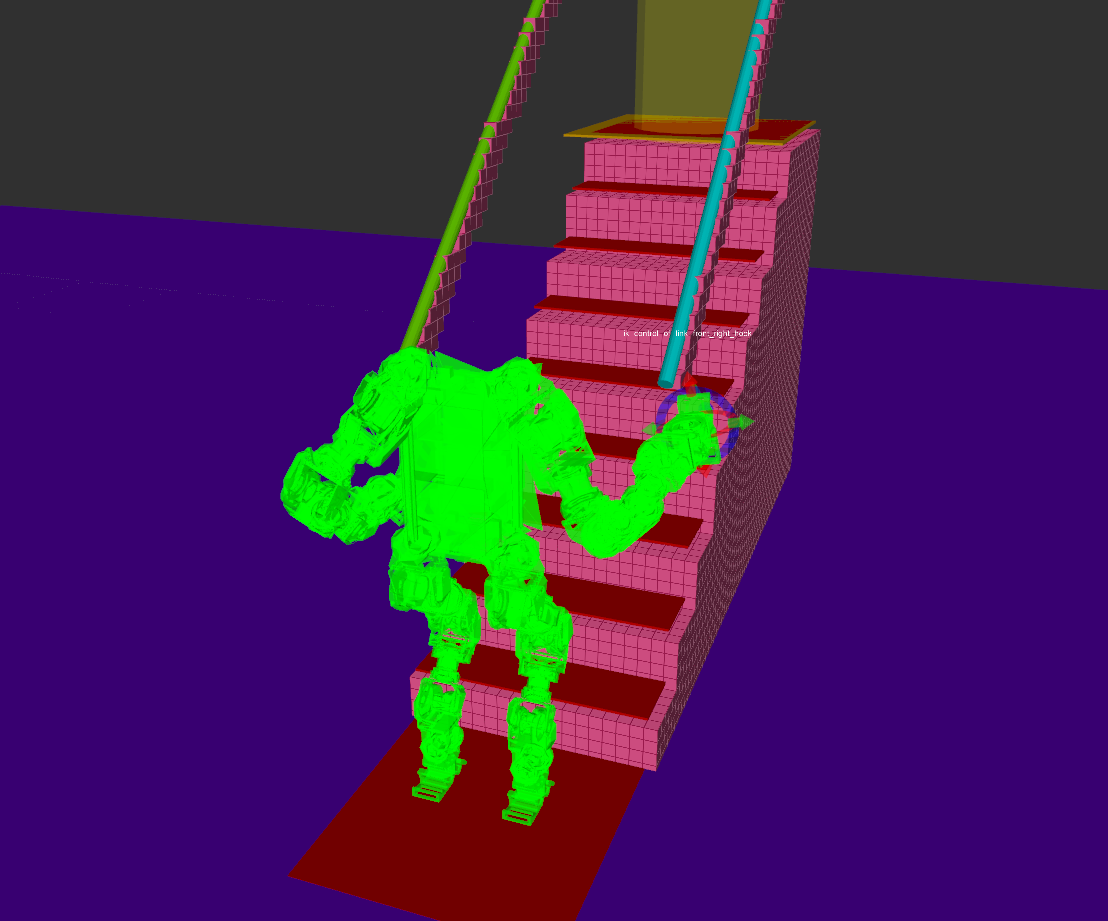
\includegraphics[width=0.283\textwidth]{fig/workspace.png}
  	\vspace{-2mm}
  \caption{
		Planning domain---Humanoid robot needs to climb the stairs while avoiding collision with the obstacles and while adhering to the physical stability constraints.
  	}
   	\label{fig:robot}
\end{figure}



%\section{Related work}
%\label{sec:related}
%

While our approach is general and can be incorporated with any motion-planning algorithm (see discussion in Sec.~\ref{}) it is especially suitable for search-based planning algorithms (see, e.g.,~\cite{CCL14}) that perform a systematic search guided by heuristic functions.
Specifically, we demonstrate it's effectiveness for the case where the motion-planning algorithm is multi-heuristic A* (MHA*)~\cite{ASNHL16, NAL15} which we detail in Sec.~\ref{sec:mha}.
%MHA* is a search-based planning algorithm that takes in multiple, possibly inadmissible heuristic functions in addition to a single consistent admissible heuristic.
%It uses them simultaneously to search the configuration space in an A*-like manner that was shown to be both complete and ensures bounds on sub-optimality. 
%This allows the search to efficiently combine the guiding powers of different heuristic functions. 


We demonstrate our approach for planning the motion of a humanoid robot. Such robots often have several dozens of degrees of freedom making planning a challenging task, especially when taking additional constraints into account such as stability and contact constraints.
One approach to plan the motion for such systems, is to use predefined, carefully chosen fixed gaits~\cite{KKKHKHAI04}. 
However, when the terrain is uneven, such planners are inadequate at computing stable motions~\cite{HBLHW08}.
Another approach is to reduce the search space by decomposing the degrees of freedom into functional groups such as locomotion and manipulation.
Then functional-specific algorithms such as footstep planning are applied to the low-dimensional space (see, e.g.,~\cite{CLCKHK05, KNKII01, PSBLY12, XCXZC09, KKNII02} for a prtial list).
A high-dimensional planner is then used to ``track'' the plan generated in the low-dimensional space.

In this work, we employ the recently-introduced adaptive dimensionality framework~\cite{GCBSL11, GSL12, GSL13}.
Roughly speaking,  it consists of two stages: an adaptive planning phase which attempts to plan in a low-dimensional space when possible and a tracking phase which plans in the high-dimensional space.
Our user-guided planner is integrated within the high-dimensional planner.

After describing our approach (Sec.~\ref{sec:planning}) we demonstrate the effectiveness of our planner (Sec.~\ref{sec:eval})
\os{finish general description}



%\subsection{Motion planning for humanoid robots}
%Our work is n
%
%
%Names that have to be mentioned:
%
%Kris K. Hauser + Timothy Bretl + Jean{-}Claude Latombe 
%Sébastien Dalibard+ Florent Lamiraux+ Jean-Paul Laumond
%
%optimization-based techniques
%
%Humanoid robots often have several dozens of degrees of freedom. Planning in such a high-dimensional space is a challenging task, especially when taking additional constraints into account such as stability and contact constraints.
%One approach, is to use a predefined, carefully chosen fixed gaits~\cite{KKKHKHAI04}. 
%However, when the terrain is uneven, such planners are inadequate at computing stable motions~\cite{HBLHW08}.
%Another approach is to reduce the search space by decomposing the degrees of freedom into functional groups such as locomotion and manipulation.
%Then functional-specific algorithms such as footstep planning are applied to the low-dimensional space (see, e.g.,~\cite{CLCKHK05, KNKII01, PSBLY12, XCXZC09, KKNII02} for a prtial list).
%A high-dimensional planner is then used to ``track'' the plan generated in the low-dimensional space.
% 
%
%%J. Chestnutt, J. Kuffner, K. Nishiwaki, and S. Kagami, “Planning biped navigation strategies in complex environments,” in Proc. IEEE Int. Conf.
%%Humanoid Robots, 2003. [CD-ROM].
%
%
%Another example is climbing a ladder. Xhang \etal~\cite{ZLHEOPPL13} generate multi-limb motion planning algorithms~\cite{12-14} by motion primitives [13], which are motions that make or break a single limb contact 
%%[12] K. Hauser, T. BretJ, and J.-c. Latombe, "Non-gaited humanoid loco­
%%motion planning," in Proc. IEEE-RAS Int. Con! on Humanoid Robots,
%%Dec. 2005, pp. 7-12.
%%[13] K. Hauser, T. Bretl, K. Harada, and J.-c. Latombe, "Using motion
%%primitives in probabilistic sample-based planning for humanoid robots,"
%%in Workshop on the Algorithmic Foundations of Robotics (WAFR), 2006.
%%[14] K. Hauser, T. BretJ, J.-c. Latombe, K. Harada, and B. Wilcox, "Motion
%%planning for legged robots on varied terrain," The International Journal
%%of Robotics Research, vol. 27, no. 11-12, pp. 1325-1349, December
%%2008.
%\subsubsection*{Motion planning}
%Perrin \etal~\cite{SBLY12}
%or fast footstep planning for legged robots on a flat ground with 3-D obstacle avoidance. We use swept volume approximations that are computed offline in order to considerably reduce the time spent in collision checking during the online planning phase, in which a rapidly exploring random tree variant is used to find collision-free sequences of half-steps (which are produced by a specific walking pattern generator). Then, an original homotopy is used to smooth the sequences into natural motions, gently avoiding the obstacles. The results are experimentally validated on the robot HRP-2.
%
%From a motion planning perspective, most motions are generated in advance based on functional
%decomposition of the degrees of freedom, for example locomotion and manipulation.
%
%
%Dalibard \etal~\cite{DKLNTL13} presents a method for planning collision-free whole-body walking motions for humanoid robots by using a randomized algorithm for constrained motion planning, that is used to generate collision-free statically balanced paths solving manipulation tasks which are transformed to collision-free dynamically balanced trajectories. 
%
%
%Kanoun \etal~\cite{KLY11} plan foot placements according to kinematic tasks addressing the question ``where should the robot place itself in order to accomplish an arbitrary kinematic goal?''
%
%Kuffner \etal~\cite{KKNII02} uses an RRT-Iike algorithm to perform a whole-body motion
%planning method that takes both obstacle avoidance as well as dynamic balance constraints into account. This is done by using a pre-computed set of statically stable postures and then
%filtering the configuration space path into a dynamically stable trajectory.
%
%
%Dalibard \etal~\cite{DNLL09} use local Jacobian-based methods within randomized motion planning.
%
%Human inspired:
%
%Mombaur \etal~\cite{MTL10} uses inverse optimal control to transfer biological motions to humanoids
%
%\subsubsection*{Manipulation}
%Dalibard \etal~\cite{DNLL10} presents a method to perform manipulation task planning
%for a humanoid robot while stepping. It introduces the concept of ``documented`` objects. Namely, objects that provide information on how to manipulate them.
\section{ALgorithmic background---MHA*}
\label{sec:mha}
\os{do we need a section detailing MHA*?}

MHA* is a search-based planning algorithm that takes in multiple, possibly inadmissible heuristic functions in addition to a single consistent admissible heuristic termed the \emph{anchor} heuristic.
It uses the the heuristic functions to simultaneously perform a set of A*-like searches that was shown to be both complete.
Using multiple heuristics allows the search to efficiently combine the guiding powers of the different heuristic functions. 

Specifically, for each search, MHA* uses a separate priority queues associated with each heuristic. 
The algorithm iterates between the search in a structured manner that ensures bounds on sub-optimality. 
This can be done in a round-robin fashion, or using more 
sophisticated approaches that allow to automatically calibrate the weight given to each heuristic~\cite{PNAL15}.

Part of the efficiency of MHA* is due to the fact that the value of the cost-to-come (the $g$-value) computed for each state is shared between all the different searches\footnote{To be precise, Aine et al.~\cite{ASNHL16} define two variants of MHA*: Independent and Shared MHA* where the queues do not share and share the $g$-values of states, respectively. In this paper when we use the term MHA* to refer to the shared variant.}.

The multiple heuristics that MHA* can use allows to automatically calibrate the weight given to each heuristic~\cite{PNAL15}.
Furthermore, using heuristics gives a principled way to identify when the planner ceases to make progress (see, e.g.,~\cite{VNL17}).

\section{Planning framework}
\label{sec:planning}
\algrenewcommand\algorithmicindent{.8em}
\begin{algorithm}[tb]
\caption{Planning framework ($\A$)}
\label{alg:main}	
\begin{algorithmic}[1]
\small
\While{$\neg\A.$\texttt{is\_solution\_found()} } 
	\While{$\neg\A.$\texttt{is\_in\_local\_minimum()}} 
		\State $\A.$\texttt{run()}
		\Comment{no user guidance}
	\EndWhile
%	
	\State {$g \leftarrow$ \texttt{get\_user\_guidance()}}
	\Comment{$\A$ is in a local minimum}
	\State $\A.$\texttt{update\_user\_guidance($g$)}
	\Comment{account for guidance}
	\While{$\A.$\texttt{is\_in\_local\_minimum()}}
		\State $\A.$\texttt{run()}
		\Comment{$\A$ uses guidance to escape local minimum}
	\EndWhile

	\State $\A.$\texttt{update\_user\_guidance($\neg g$)}
	\Comment {remove  guidance}
\EndWhile
\end{algorithmic}
\end{algorithm}

\subsection{High-level approach}
\label{sec:high}
To employ our planning framework, we assume that we are given a motion-planning algorithm $\A$ that is endowed with two non-standard procedures which are planner dependent.
The first, \texttt{is\_in\_local\_minimum()}, 
identifies when it is in a \emph{local minimum}, namely when $\A$'s search does not progress towards the goal. 
The second, \texttt{update\_user\_guidance()}, 
incorporates (or removes) the user guidance provided to $\A$. 

Equipped with these functions, we can describe our planning framework, detailed in Alg.~\ref{alg:main}.
The framework runs as long as no solution is found (line~1).
It runs the planner~$\A$ (lines~2-3) as long as it continuously makes progress towards the goal (namely, it is not in a local minima).
Once a local minima is identified, user guidance is invoked (line~4) and $\A$  is updated to make use of this guidance (line~5).
It is then run while using the guidance as long as it is still in the local minima (lines~6-7).
Once it escapes the local minima $\A$ is updated to remove the guidance that was provided by the user (line~8).


We demonstrate our planning framework for the case where the motion-planning algorithm $\A$ is multi-heuristic A* (MHA*)~\cite{ASNHL16}.
%MHA* is a search-based planning algorithm that takes in multiple, arbitrarily inadmissible heuristic functions in addition to a single consistent heuristic.
%It uses them simultaneously to search the configuration space in an A*-like manner that was shown to be both complete and ensures bounds on sub-optimality. 
%This allows the search to efficiently combine the guiding powers of different heuristic functions. 
For a visualization of the way the algorithm progresses, see Fig.~\ref{fig:filmstrip-dynamic_heuristic}.

Our implementation is slightly more complicated than that described in Alg~\ref{alg:main}.
Specifically, the planner can be in a local minima in the dynamically-generated queue that is used to escape the original local minima. 
In such cases we request new guidance from the user and replace the previous guidance with the new one.

\begin{figure*}[t]%
%\captionsetup{format = plain}
  \centering%
  \subfigure[]
  {
  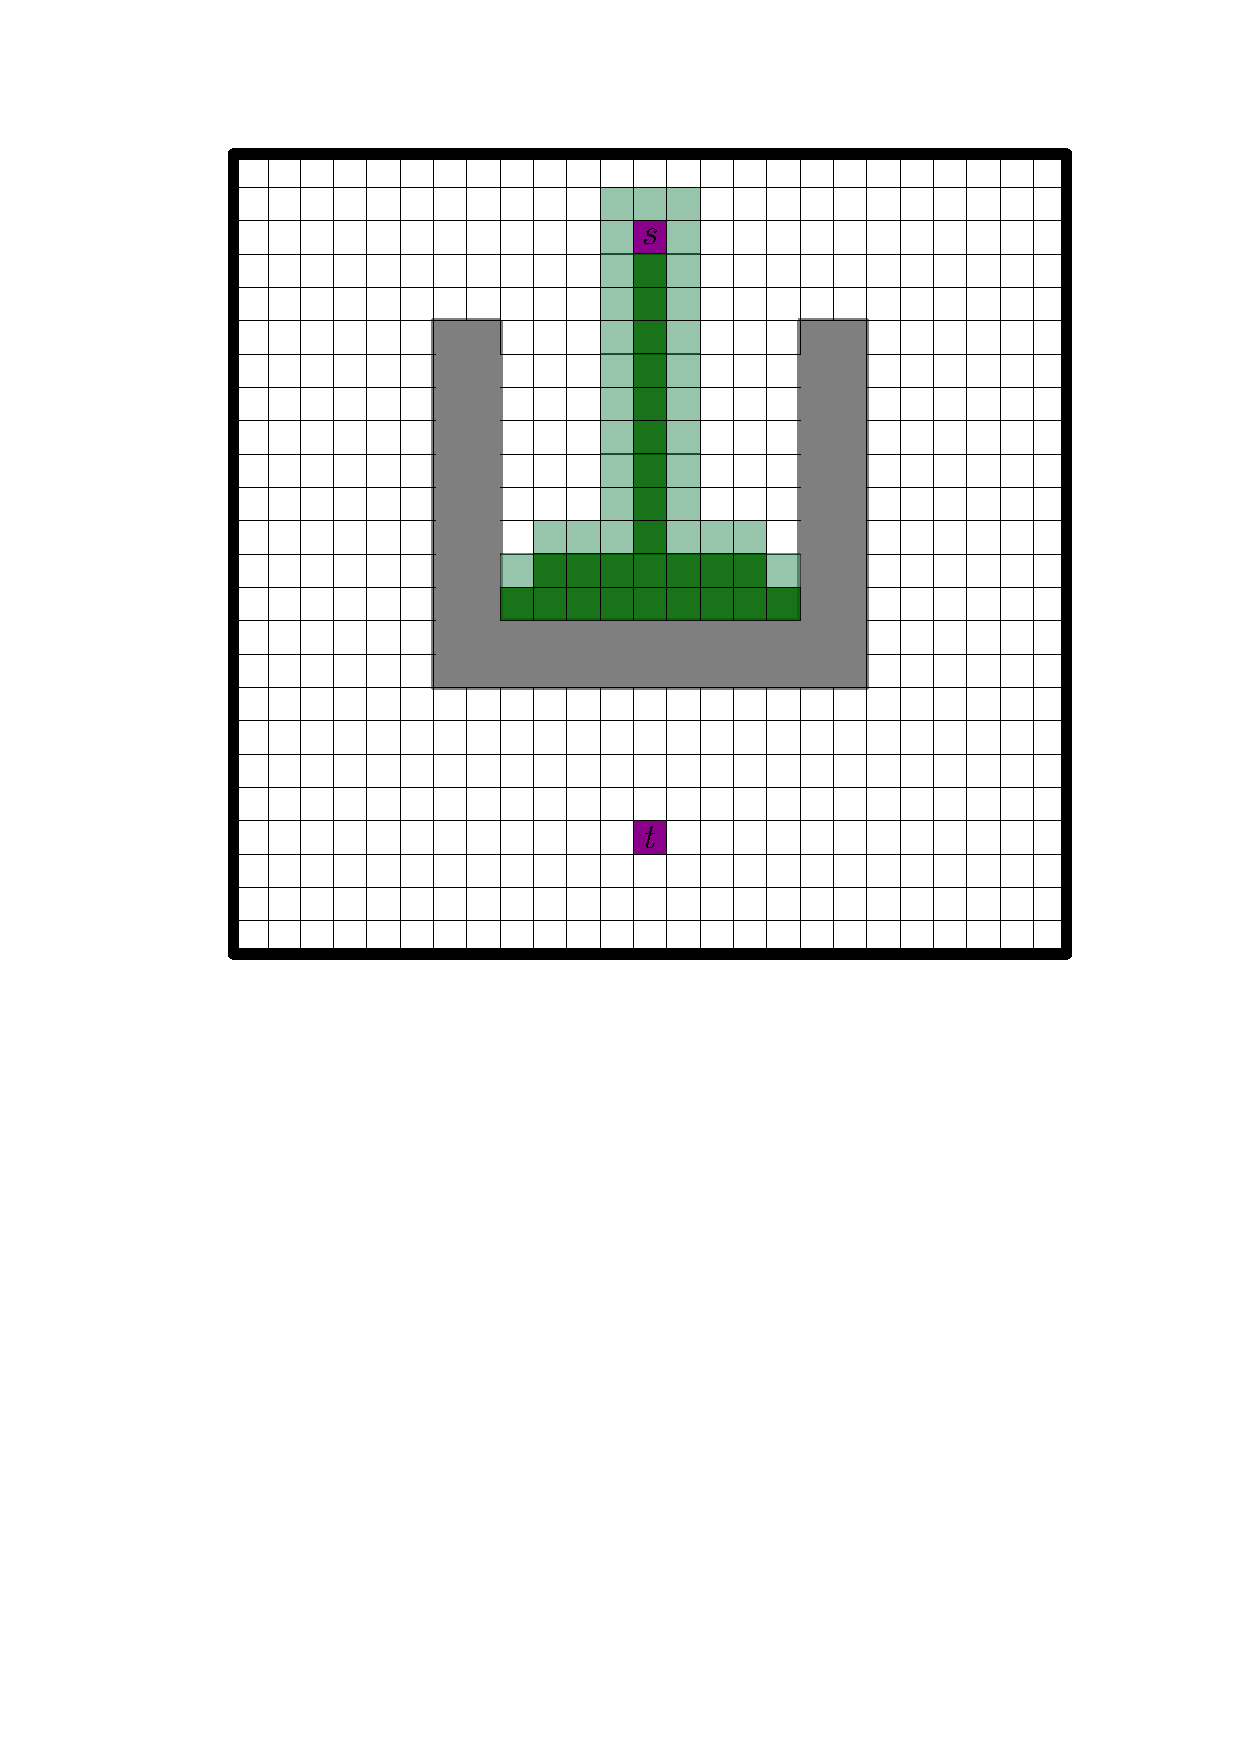
\includegraphics[width=0.225\textwidth]{fig/example_1.pdf}
  \label{fig:dynamic_heuristic1}
  }
  \subfigure[]
  {
  \label{fig:dynamic_heuristic2}
  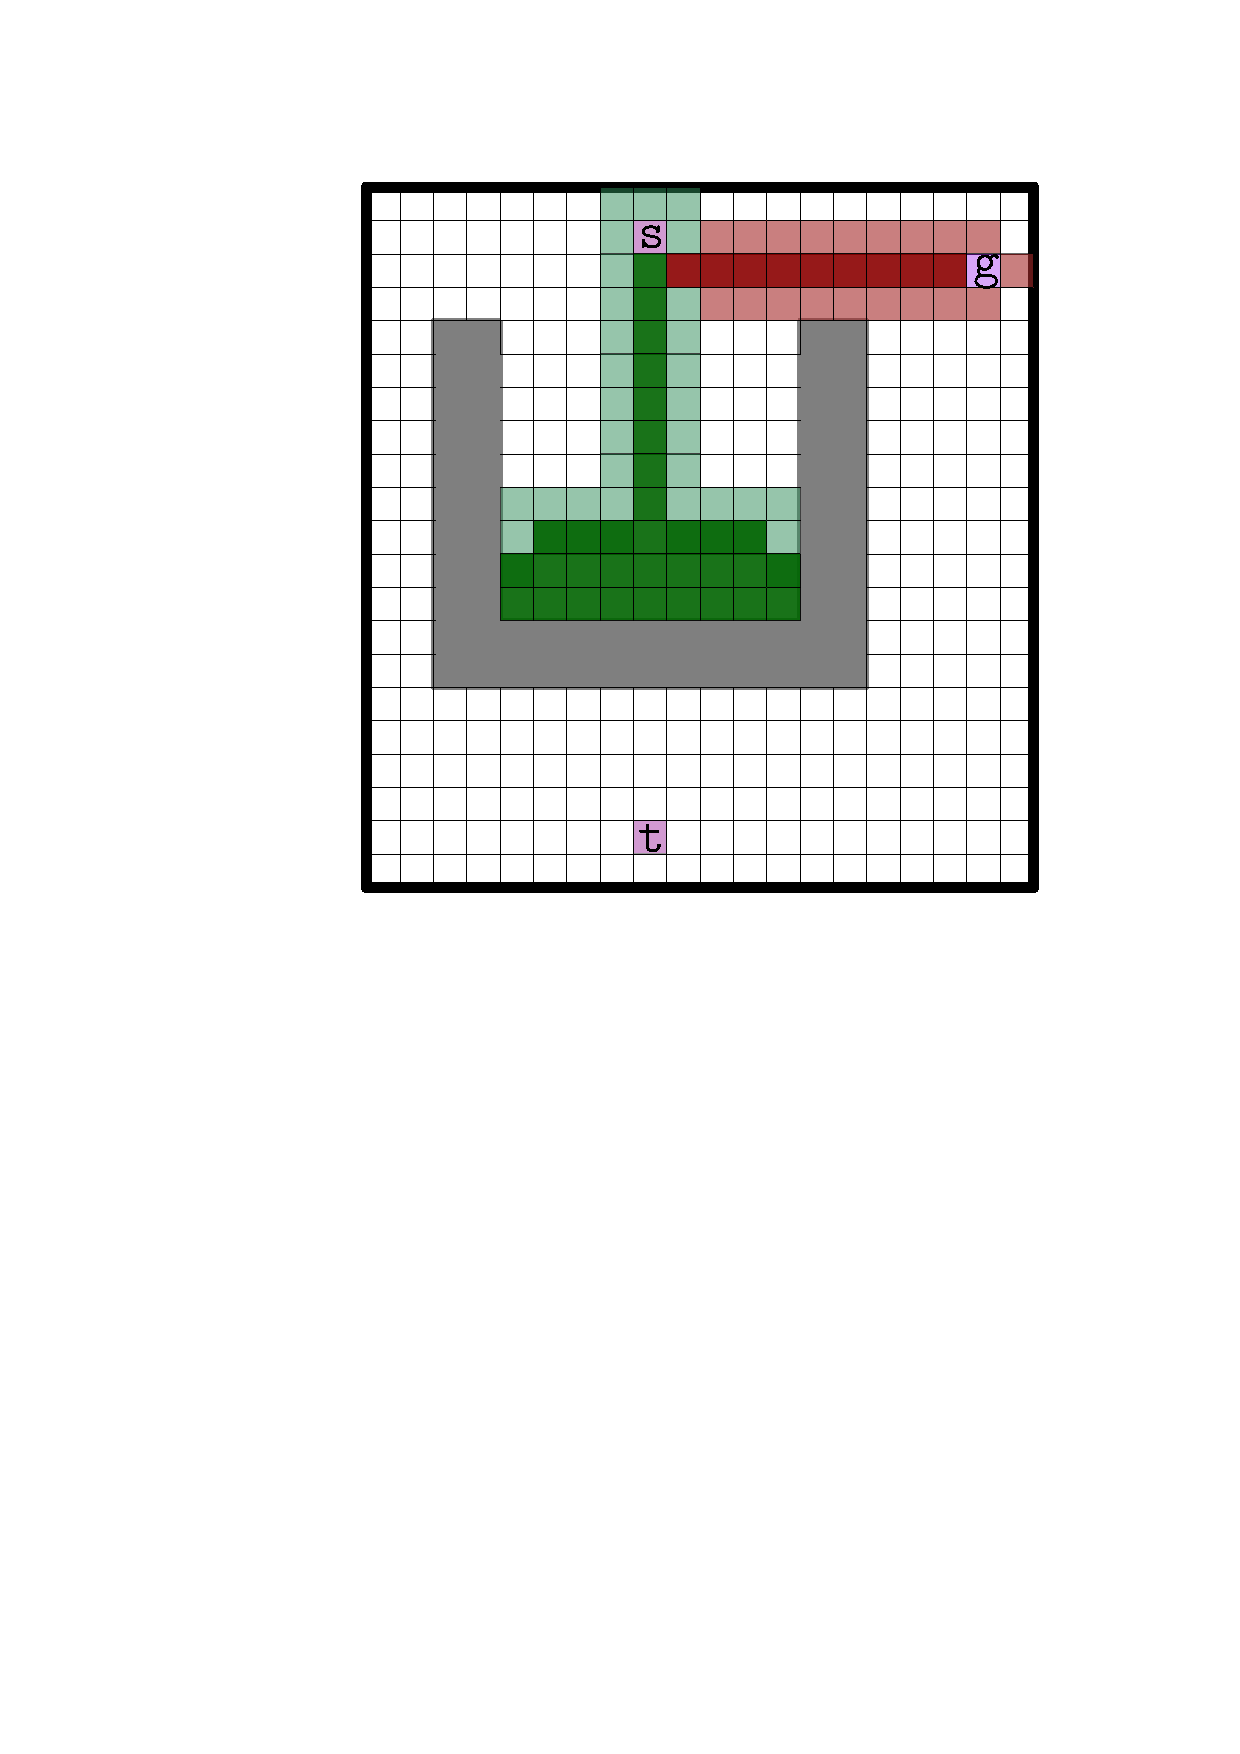
\includegraphics[width=0.225\textwidth]{fig/example_2.pdf}
  }
  \subfigure[]
  {
  \label{fig:dynamic_heuristic3}
  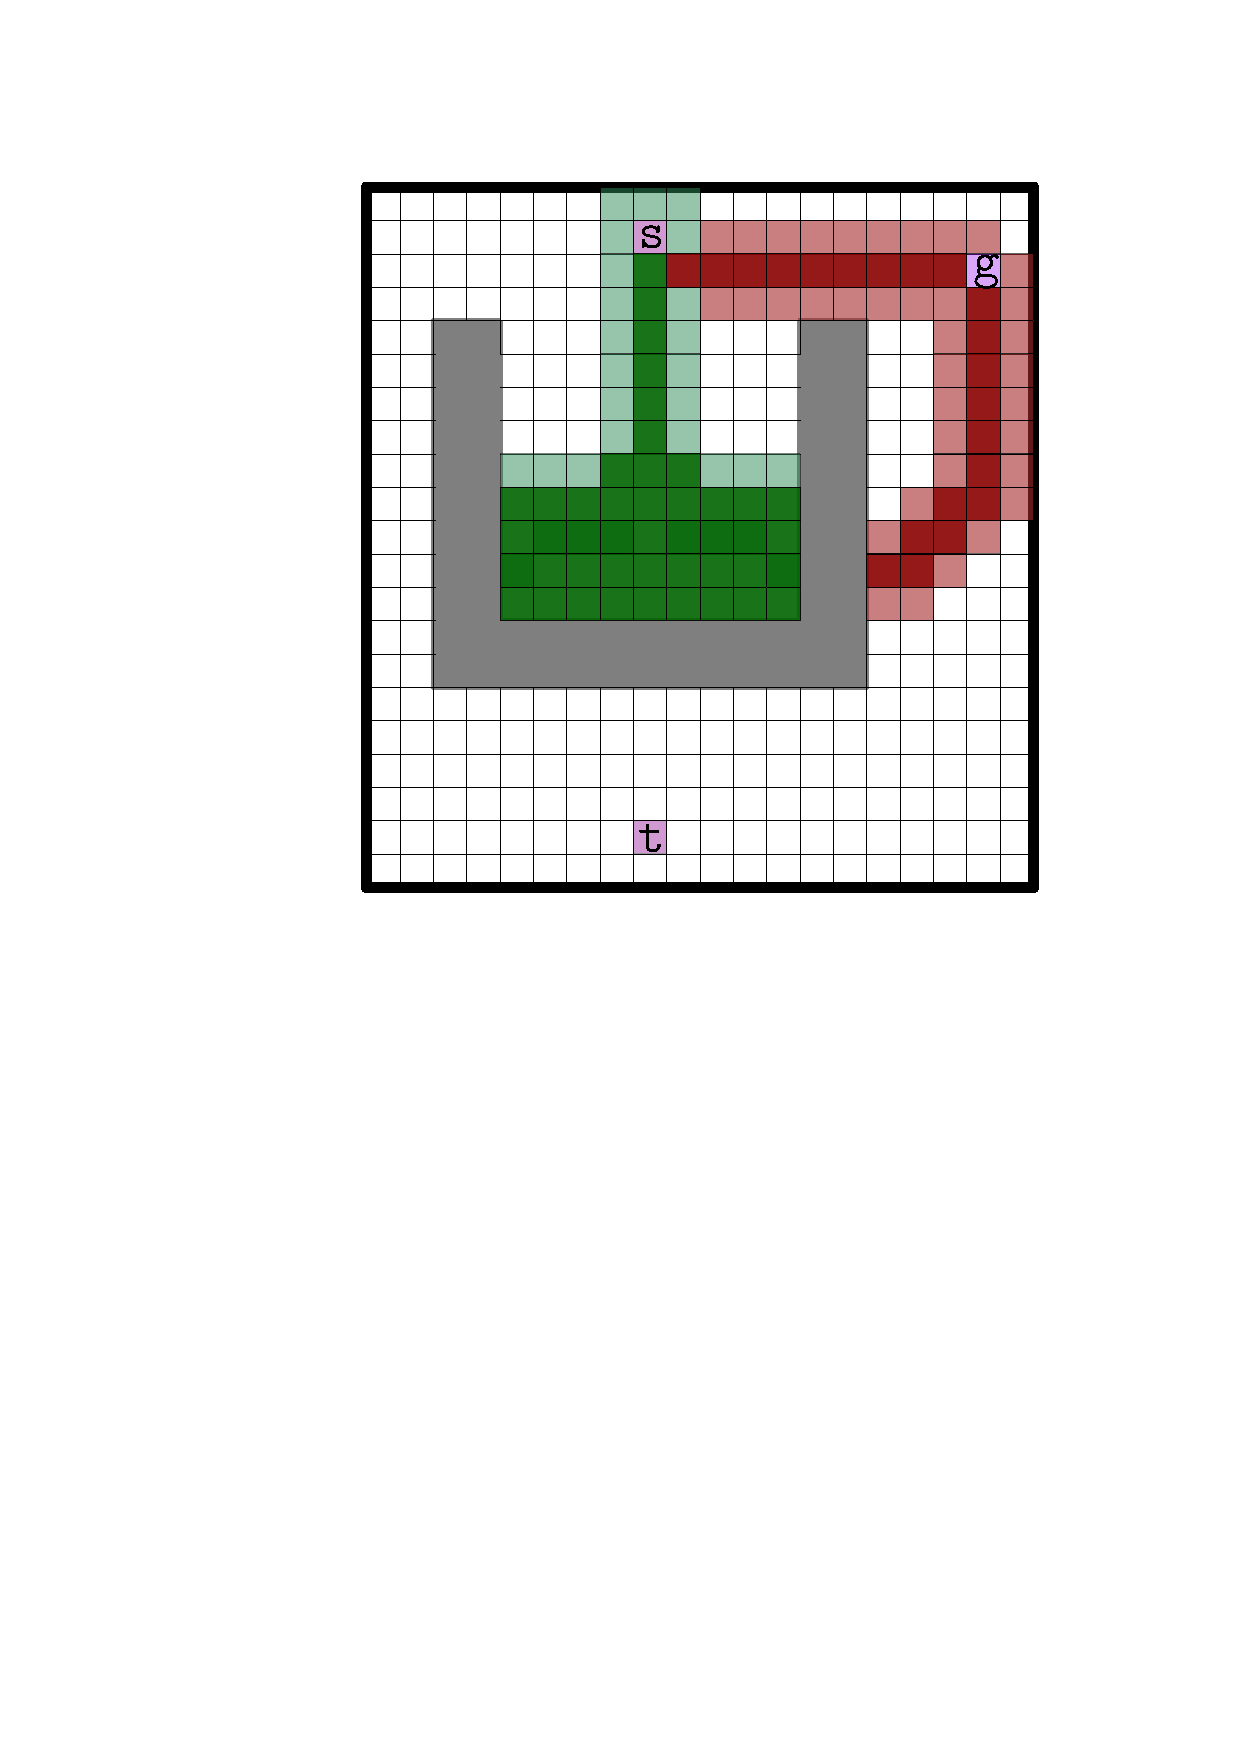
\includegraphics[width=0.225\textwidth]{fig/example_3.pdf}
  }  
  \subfigure[]
  {
  \label{fig:dynamic_heuristic4}
  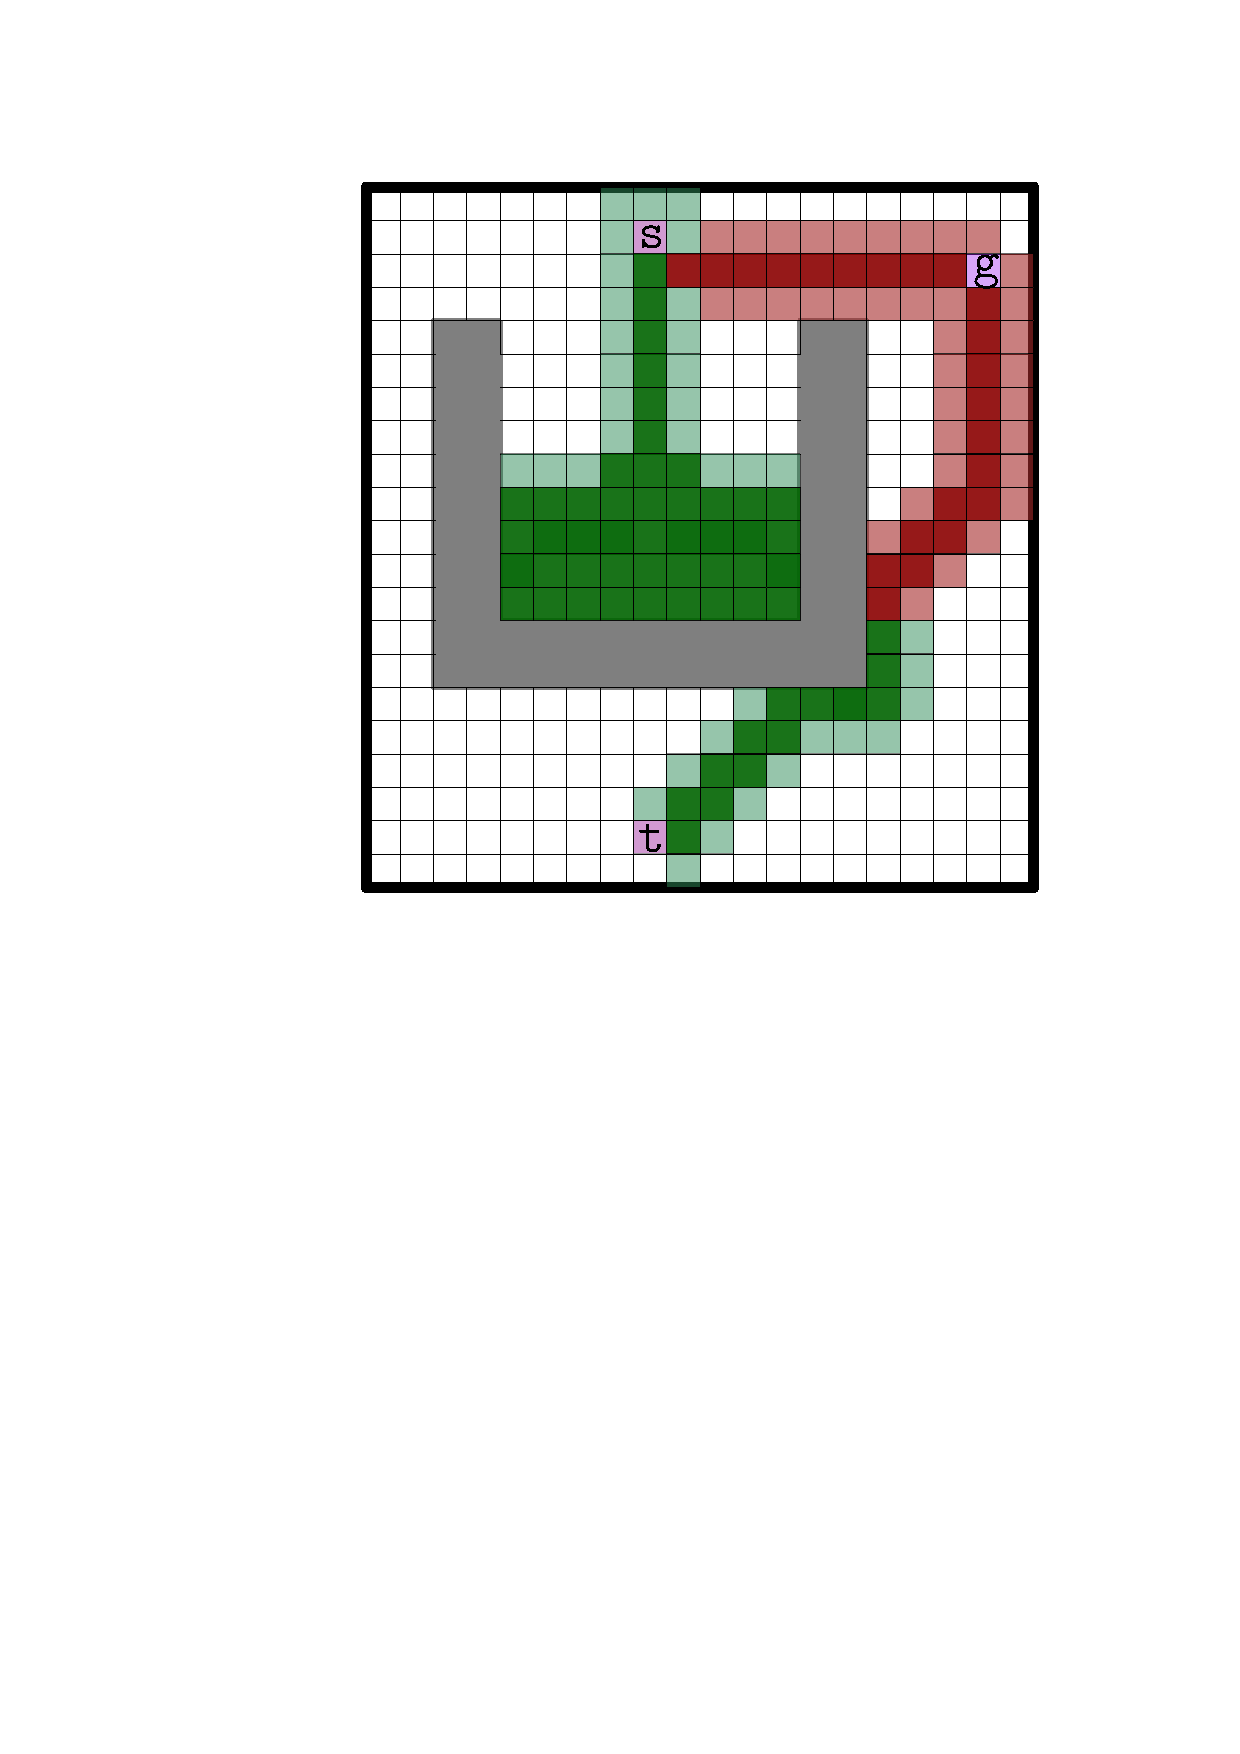
\includegraphics[width=0.225\textwidth]{fig/example_4.pdf}
  }
  \caption{%
    Algorithm progression.
    States popped from a priority queue are depicted using dark colors while states still in a queue are depicted by a light color.
    Start, target and user-guided states are depicted in purple with the letters \texttt{s}, \texttt{t}, \texttt{g}, respectively. 
    %
    In this example MHA* is implemented using shared queues and alternating between queues in a round-robin fashion. Furthermore, heuristics are inflated by a weight of $w=\infty$. Namely, the priority queues are ordered according to the heuristic-value of the states.
    %
	\subref{fig:dynamic_heuristic1}~MHA* starts with the single anchor heuristic (green) which is the Euclidean distance to goal and a local minimum is identified.
    %
	\subref{fig:dynamic_heuristic2}~User provides guidance and the algorithm automatically generates an additional heuristic (red) that drives the search towards the guidance (notice that the anchore heuristic continues to search the local minimum).
    %
	\subref{fig:dynamic_heuristic3}~After passing through the guidance, the additional heuristic (red) drives the search towards the goal.
    %
	\subref{fig:dynamic_heuristic4}~After the additional heuristic found states that are at the top of the priority queue of the anchor heuristic, the additional heuristic is deleted and the anchor heuristic drives the search towards the goal.
  }%
  \label{fig:filmstrip-dynamic_heuristic}%
  \vspace{-2.5mm}
\end{figure*}


\subsection{Invoking user guidance}
\label{sec:q1}

\begin{figure*}[t]%
%\captionsetup{format = plain}
  \centering%
  \subfigure[]
  {
  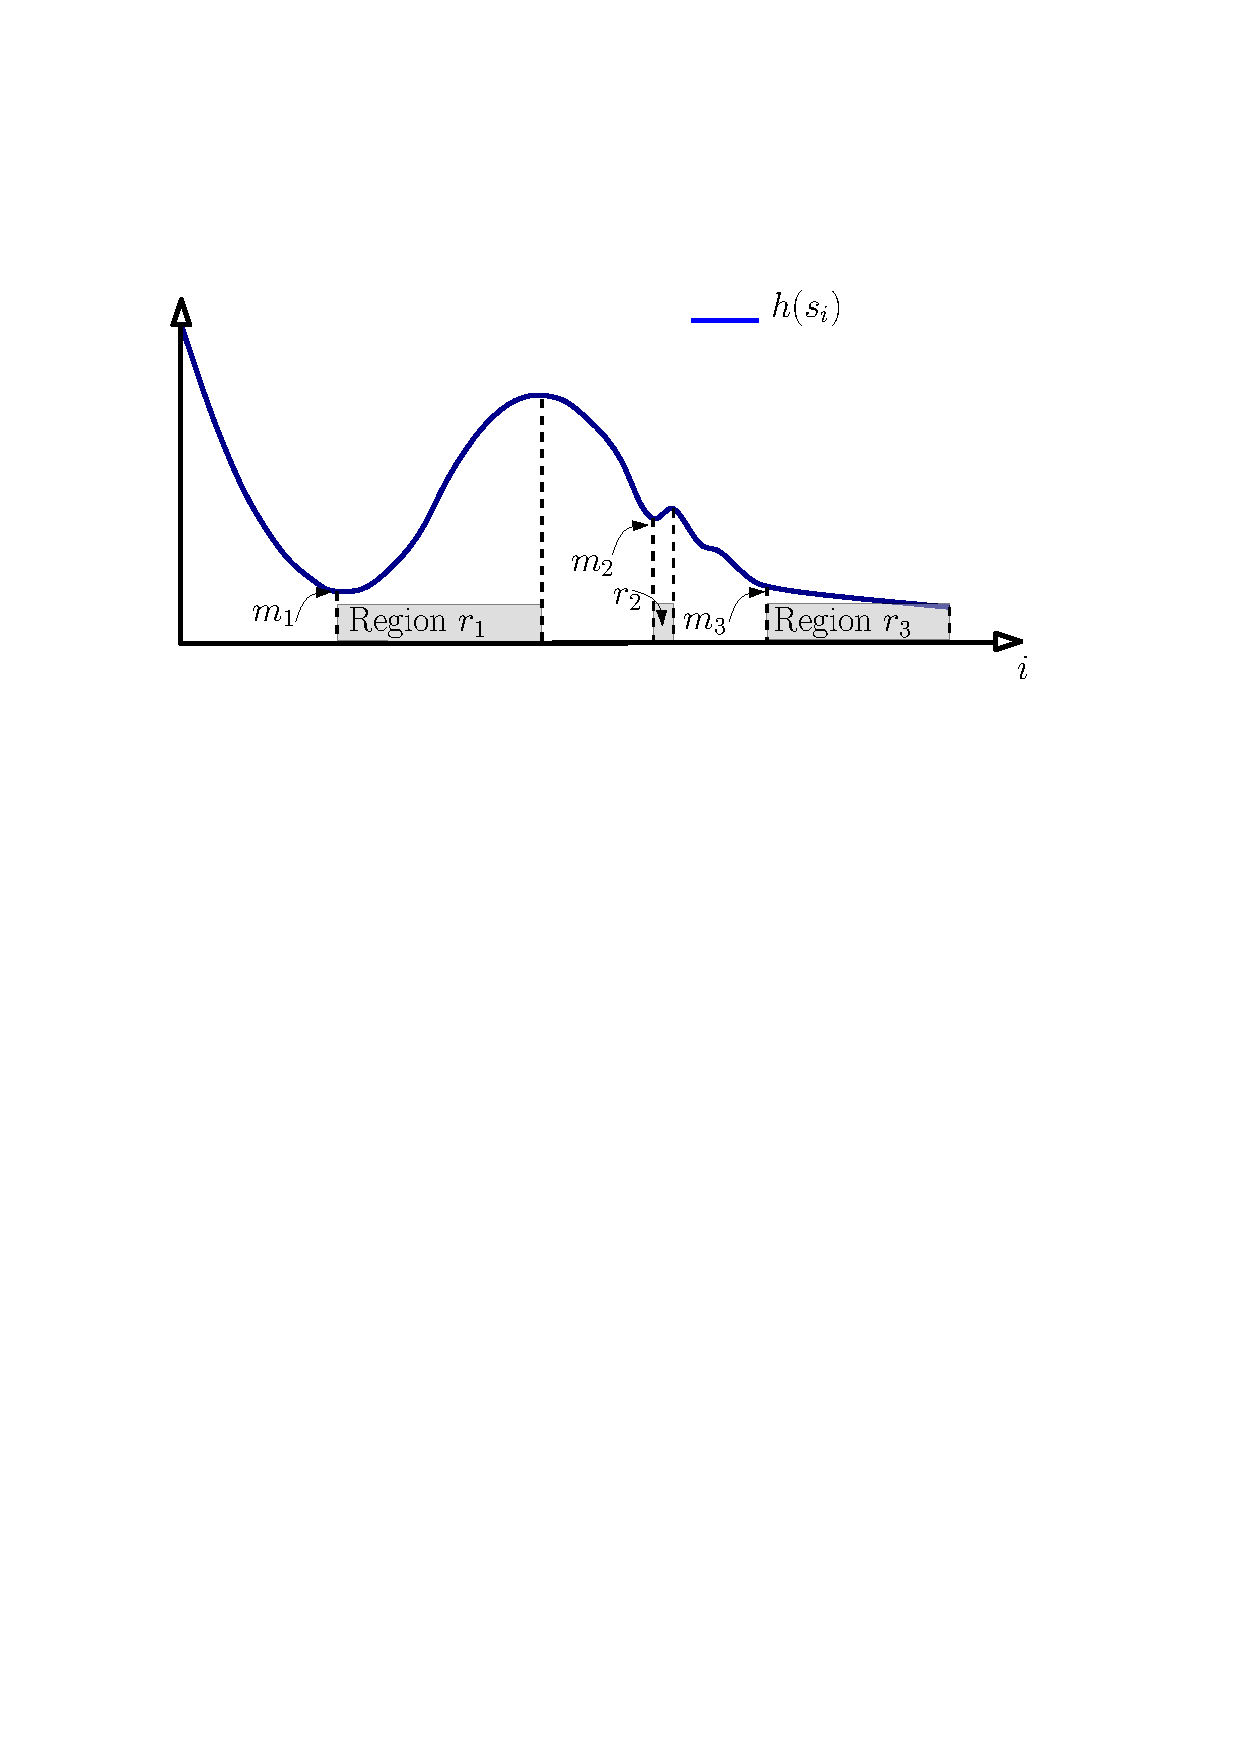
\includegraphics[width=0.34\textwidth]{fig/local_min_detection_1.pdf}
  \label{fig:local_min1}
  }
  \hspace{-10mm}
%  \subfigure[]
%  {
%  \label{fig:local_min2}
%  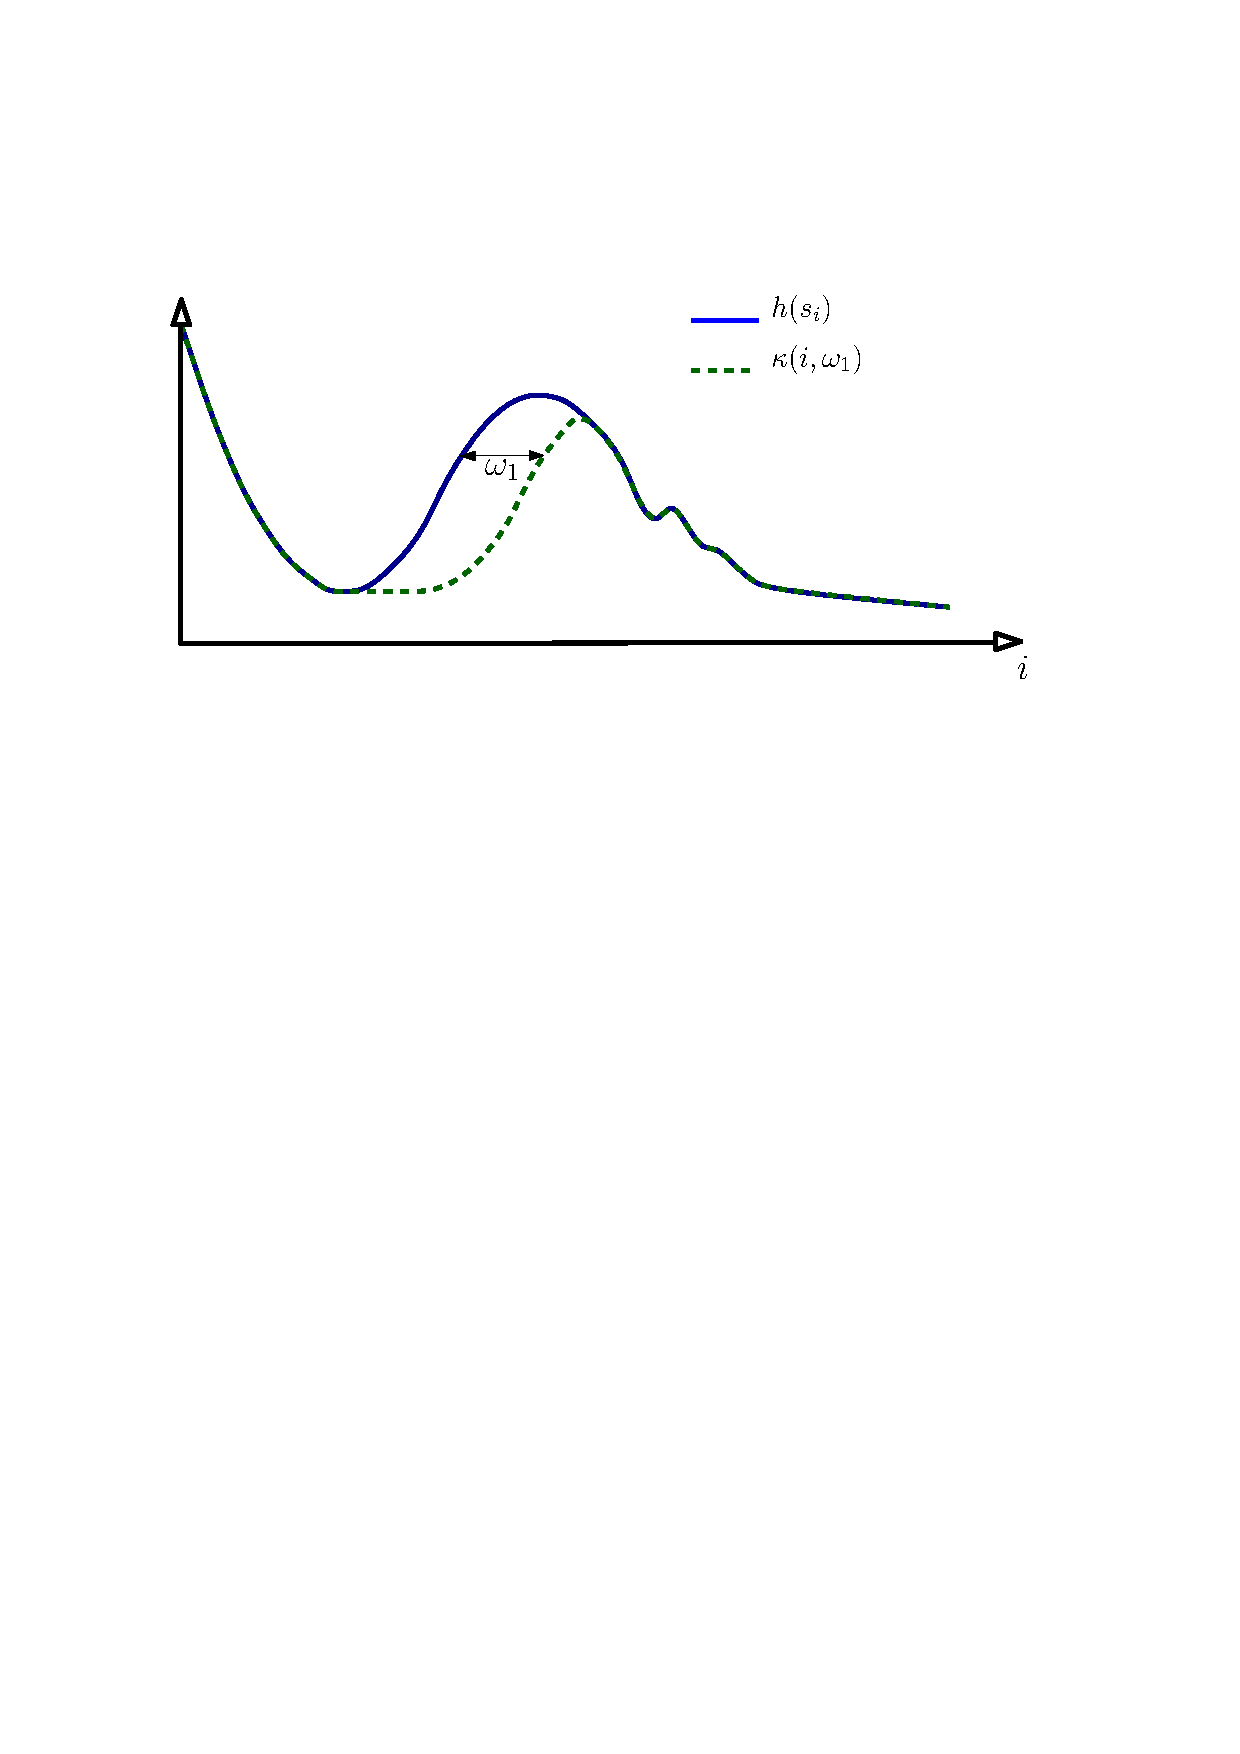
\includegraphics[width=0.265\textwidth]{fig/local_min_detection_2.pdf}
%  }
%  \hspace{-10mm}
  \subfigure[]
  {
  \label{fig:local_min3}
  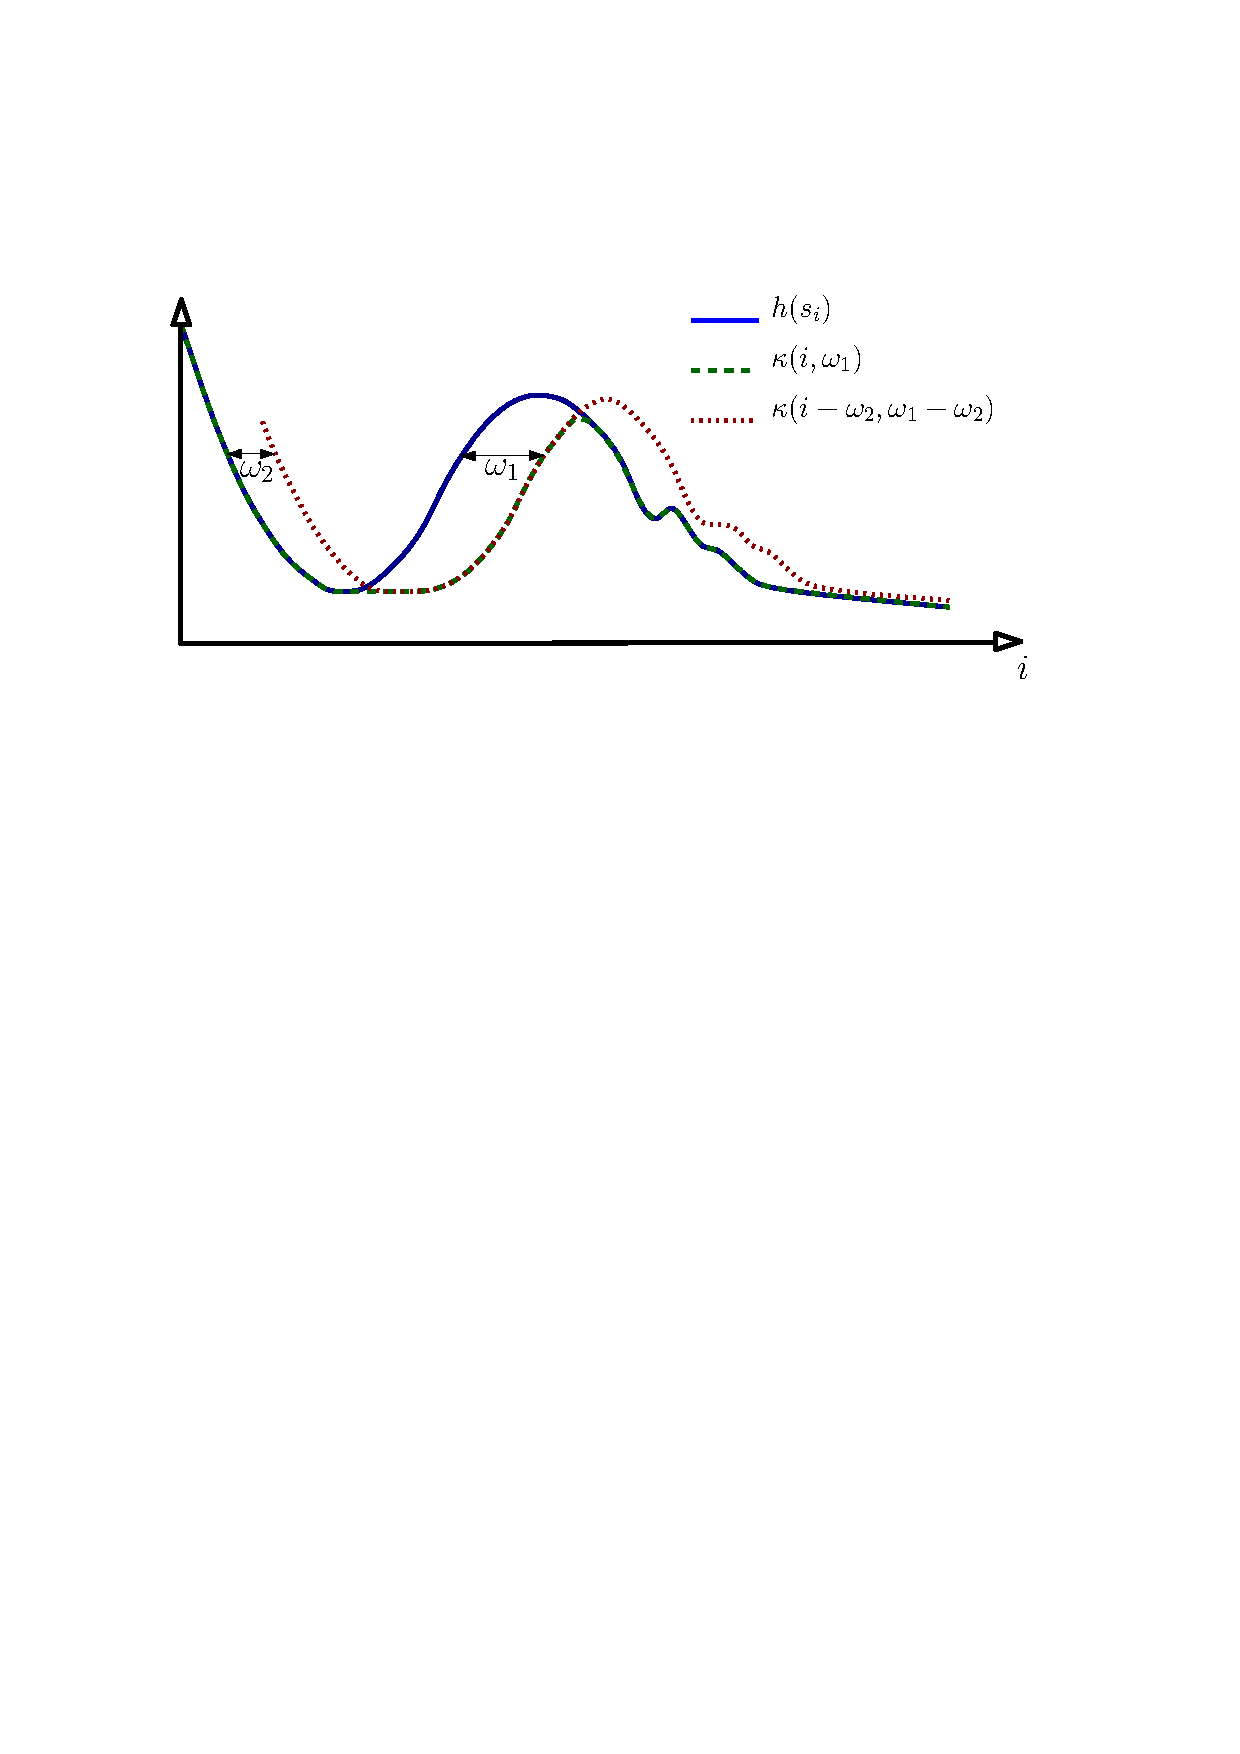
\includegraphics[width=0.34\textwidth]{fig/local_min_detection_3.pdf}
  }  
  \hspace{-10mm}
  \subfigure[]
  {
  \label{fig:local_min4}
  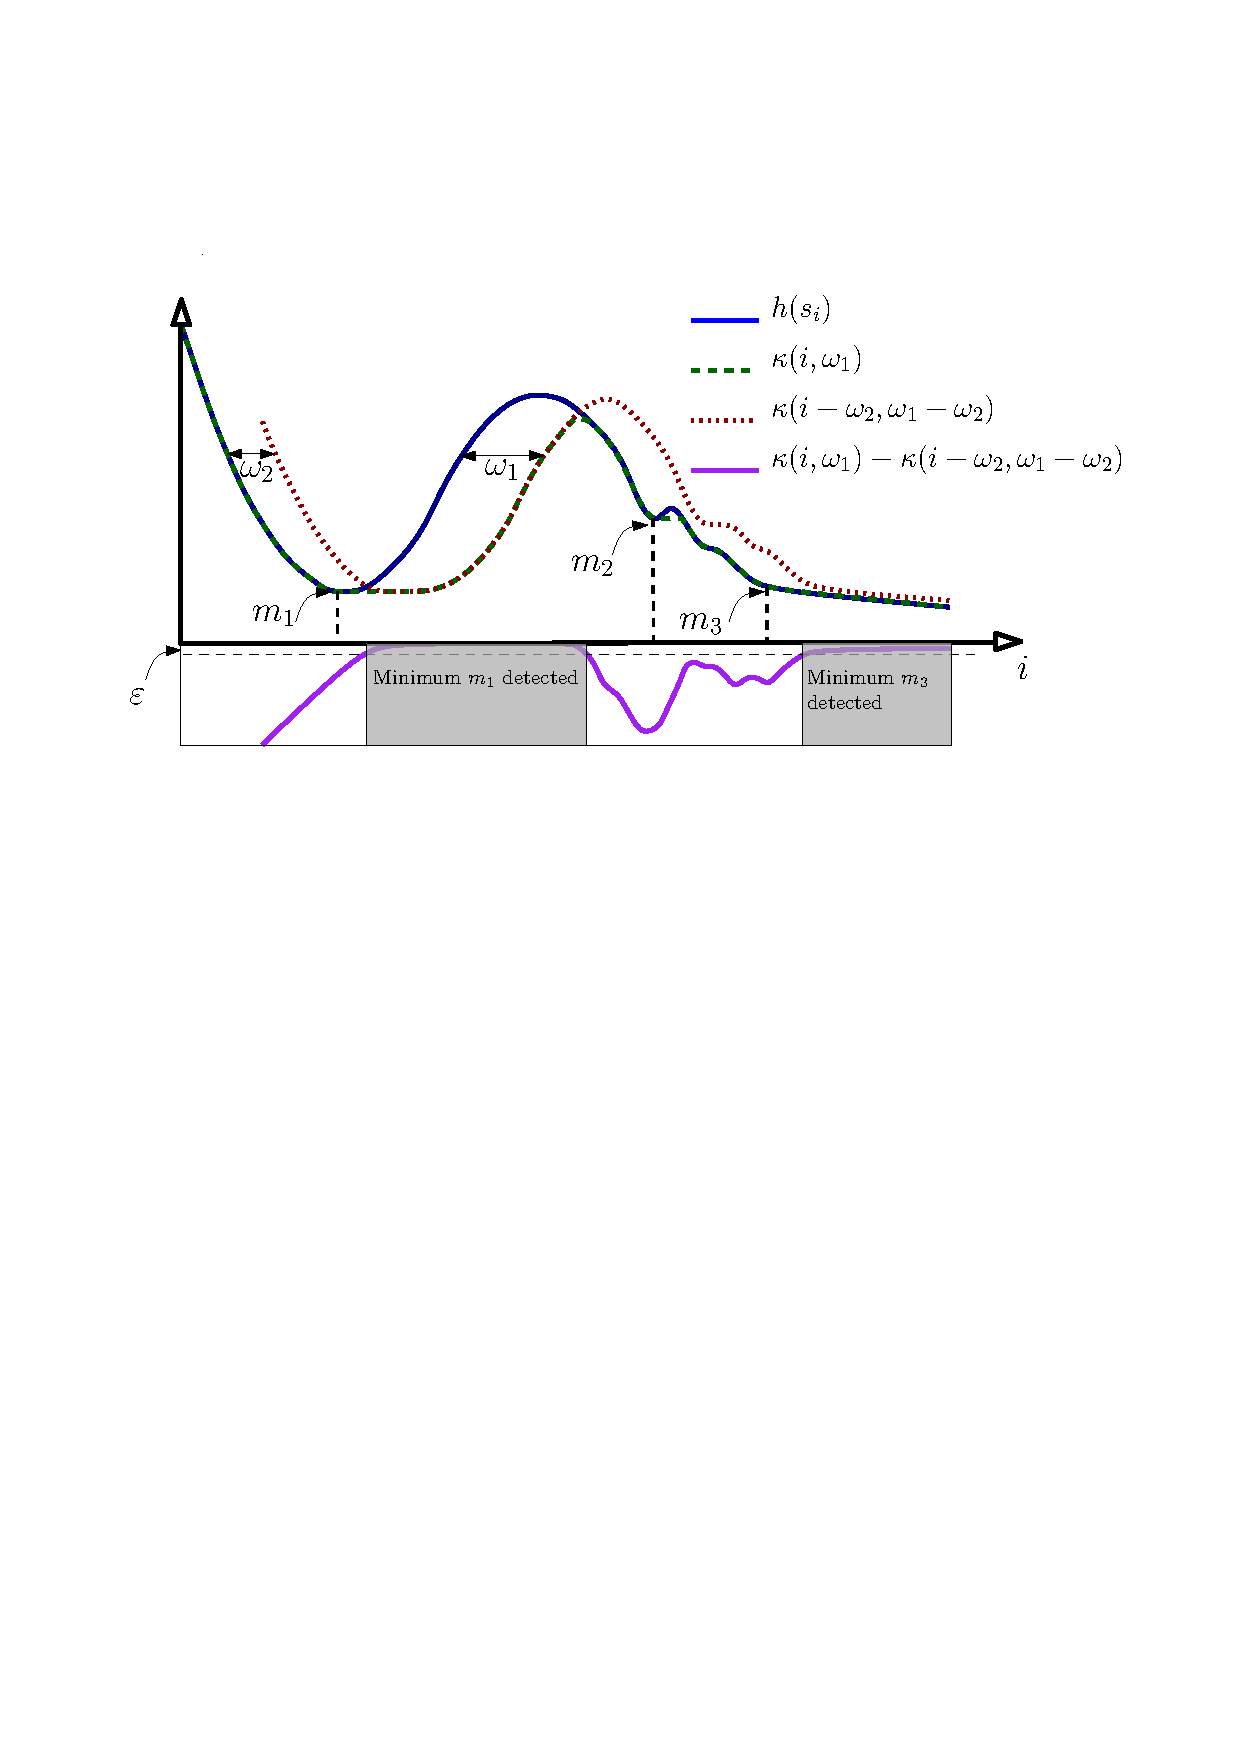
\includegraphics[width=0.34\textwidth]{fig/local_min_detection_4.pdf}
  }
  \caption{%
    Visualization of the way stagnation regions are detected.   
	\subref{fig:local_min1}~The heuristic value $h(s_i)$ (solid blue) has three local minima, $m_1, m_2$ and $m_3$ followed by three stagnation regions (light grey). Local minima $m_2$ is very small while~$m_3$ is not a local minimum per se, yet the progress made between consecutive steps is smaller than the predefined threshold~$\varepsilon$.
    %
%    \subref{fig:local_min2}~
	The function $\kappa(i,\omega_1)$ (dashed green) returns the minimal value $h(s_i)$ attained over the past~$\omega_1$ iterations (referred to  as the ``recent history'').
    %
    \subref{fig:local_min3}~The function $\kappa(i-\omega_2,\omega_1-\omega_2)$ (dotted red) returns the minimal value $h(s_i)$ attained over the beginning of the recent history.
    %
    \subref{fig:local_min3}~The difference between the two functions (solid purple) indicates if there was significant progress (i.e. more than $\varepsilon$) made at the end of the recent horizon when compared to the beginning of the recent history. 
    If not, then the planner detects a stagnation region (dark grey).
		Notice that the hysteresis parameters~$\omega_1$ and $\omega_2$ 
		(i)~induce a lag from the time that the stagnation region starts until it is detected,
		(ii)~allow to avoid detecting a stagnation region~$r_2$.  
		}%

  \label{fig:filmstrip-local-min}%

  \vspace{-2.5mm}

\end{figure*}





%\begin{figure}[tb]
%  \centering
%  	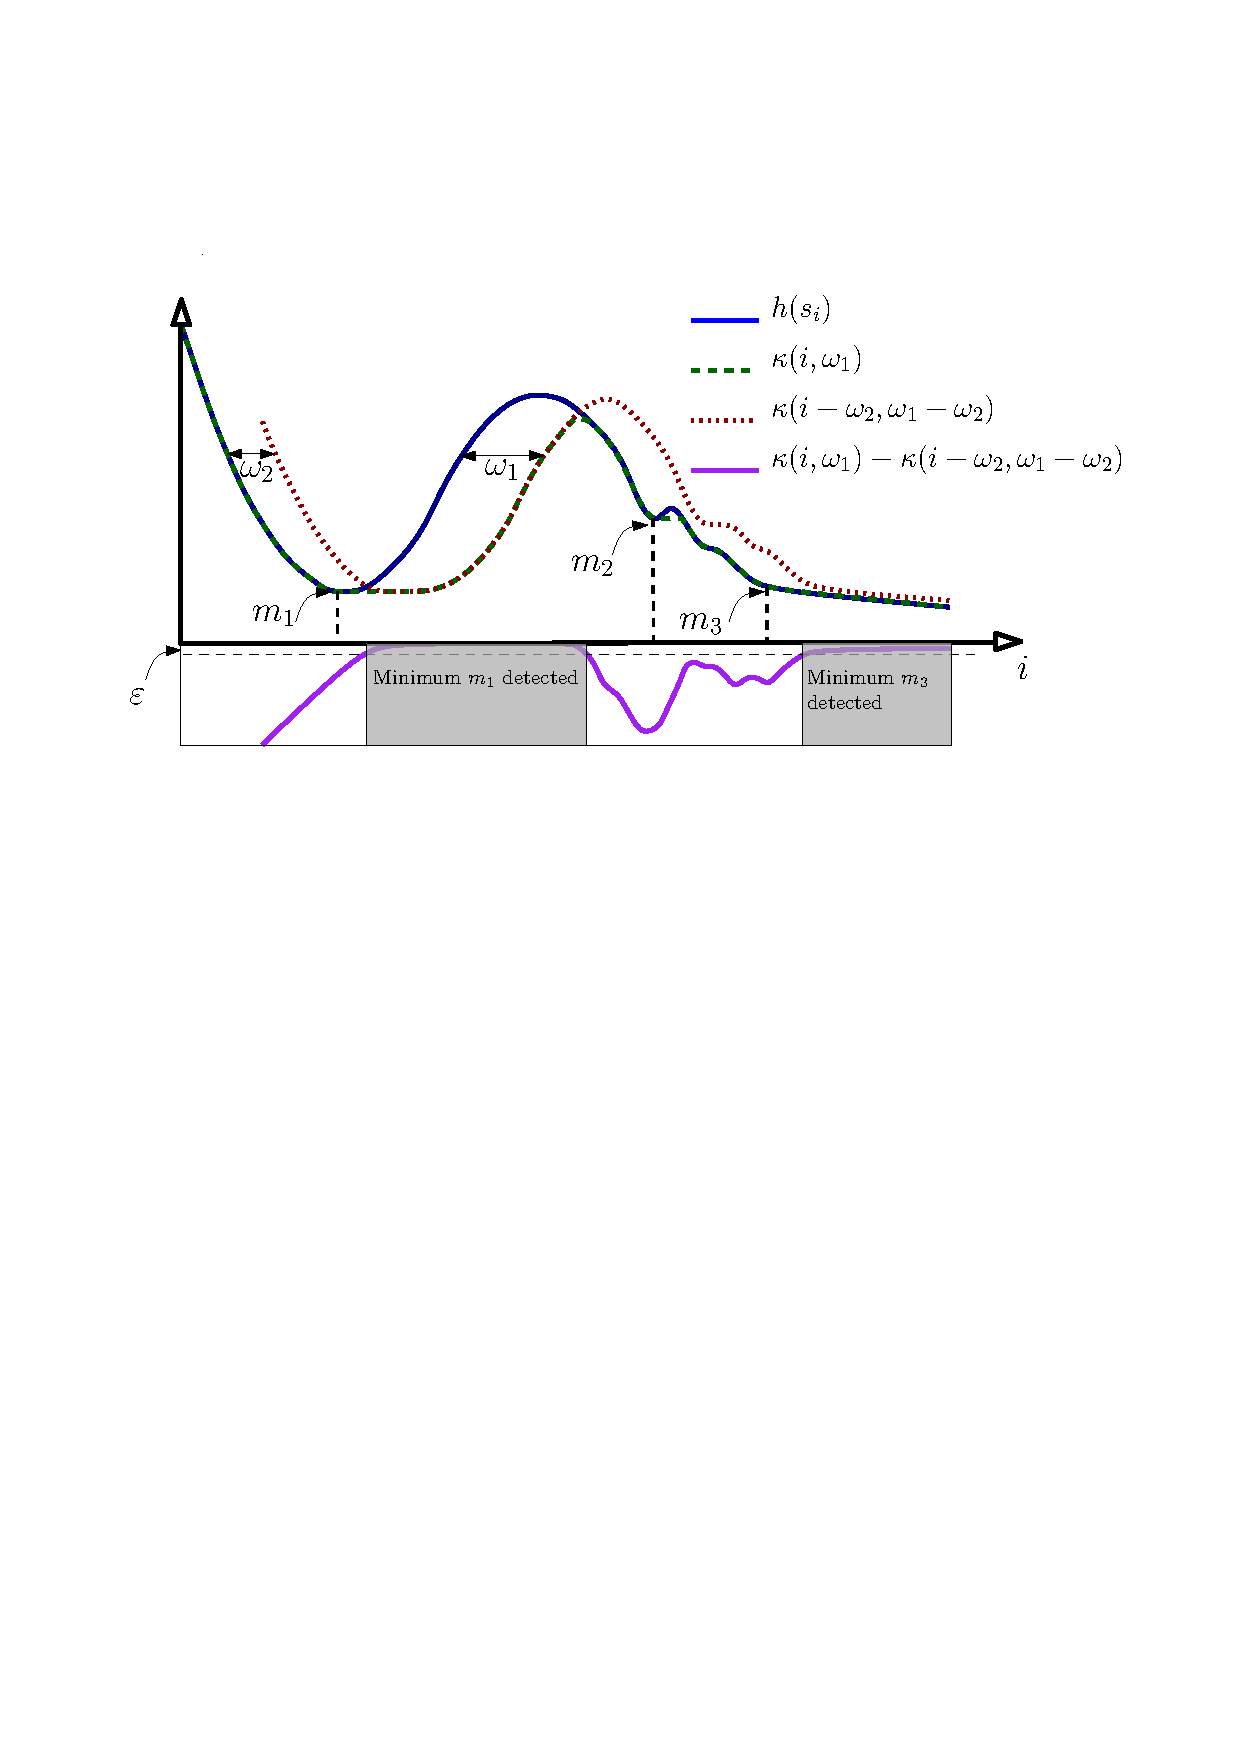
\includegraphics[width=0.49\textwidth]{fig/local_min_detection_4.pdf}
%  	\vspace{-5mm}
%  \caption{
%		Visualization of the way local minima are detected.
%		The heuristic value $h(s_i)$ has three local minima, $m_1, m_2$ and $m_3$.
%		Local minima $m_2$ is very small while~$m_3$ is not a local minimum per se, yet the progress made between consecutive steps is smaller than the predefined threshold~$\varepsilon$.
%		When the value of $\kappa(i,w) -  \kappa(i-\omega_2,\omega_1-\omega_2)$ is larger than $\varepsilon$, a local minimum is detected, visualized by a gray region.
%		Notice that the hysteresis parameters~$\kappa_1$ and $\kappa_2$ 
%		(i)~induce a lag from the time that the minimum occurs until it is detected,
%		(ii)~allow to avoid detecting minimum $m_2$.		
%  	}
%   	\label{fig:robot}
%  	\vspace{-5mm}
%\end{figure}

The heuristic functions of search-based planning algorithms, such as MHA*, can be used to estimate in a principled manner when the planner is in a local minimum (Alg~\ref{alg:main}, lines 2, 6). 
%Specifically, in such algorithms,  we proceed by iteratively choosing  the current-best state from a priority queue and computing all its successors. 
%
We suggest to identify when the planner is in a local minimum as follows:
Let~$\Q$ be a priority queue 
ordered according to some heuristic function~$h_\Q(\cdot)$,
$s_i$ be the node expanded from~$\Q$ at the $i$'th iteration and $\omega_1, \omega_2$ be parameters such that $\omega_1 > \omega_2$.
%
We define 
$\kappa_\Q(i, \omega) = \min_{i-\omega \leq j \leq i} \{ h_\Q(s_j)\}$.
Namely, $\kappa_\Q(i, \omega)$ denotes the minimal value attained by $h_\Q$ in the past~$\omega$ states. 
%
\begin{definition}
A queue~$\Q$ is defined to be in a local minimum if 
$\kappa_\Q(i, \omega_1) \geq \kappa_\Q(i - \omega_2, \omega_1 - \omega_2) - \varepsilon$.
\end{definition}
\noindent Namely~$\Q$ is in a local minimum if looking at the previous~$\omega_1$ iterations, 
there was no reduction 
(by more than some threshold $\varepsilon$) 
in the minimum value of~$h_\Q$ 
in the last $\omega_2$ states expanded from $\Q$.

\begin{definition}
MHA* is defined to be in a local minimum if 
all it's queues are in local minima.
\end{definition}

Thus, our algorithm is given three additional parameters~$\omega_1, \omega_2$ and $\varepsilon$ 
and implements the function \texttt{is\_in\_local\_minimum()} by maintaining for each queue~$\Q$ the values 
$\kappa_\Q(i, \omega_1)$ and $\kappa_\Q(i - \omega_2, \omega_1 - \omega_2)$.
Note that testing if a single queue is in a local minimum takes $O(1)$ time.




%
%$\{h_\Q(s(i-\omega)), \ldots h_\Q(s(i))\}$ to be the minimum heuristic value attained by the last $\omega$ nodes that were expanded from~$\Q$ (assuming we are at the $i$'th iteration).
%We will say that the planner is in a local minima for $\Q$ if 
%$\kappa_\Q(\omega,i) \geq \kappa_\Q(\omega,i-1) - \varepsilon$.
%Namely, if there was no reduction 
%(by more than some threshold $\varepsilon$) 
%in the minimum value of~$h_\Q$ in the last $\omega$ states expanded from $\Q$.

%
%
%
%\os{possibly remove next paragraph}
%
%Once a local minimum is identified, should we immediately ask for user guidance? If we are in a shallow local minima, providing the planner with additional computation time (possibly much shorter than the time required by the user to produce guidance) may be sufficient.
%This is an example of the ski rental problem~\cite{KMMO94} in which there is a tradeoff between continuing to pay a repeating cost (letting the algorithm try to escape its local minima) or paying a one-time cost which eliminates or reduces the repeating cost (invoking user guidance).
%By using a randomized approach we can obtain a $\frac{e}{e-1}\approx1.58$ competitive ratio\footnote{The competitive ratio of an online algorithm \texttt{ALG} is the ratio between the performance of \texttt{ALG} and the performance of an optimal offline algorithm.}~\cite{KMMO94}.
%Indeed, this approach has already been used to identify when robots should ask for help from a user~\cite{RV12}.

\subsection{Form of user guidance}
\label{sec:q2}
We chose to obtain user guidance 
(Alg~\ref{alg:main}, line~4)
in the form of an intermediate configuration $\hat{q}$ that is used to guide the planner. We discuss alternative options in Sec~\ref{sec:eval}.

The framework includes a graphical user interface (GUI) capable of  depicting the robot and the workspace.
Once user guidance is invoked, 
a configuration in the local minima is obtained and the robot is placed in that configuration (as well as the start configuration and target region) in the GUI.
This allows the user to try and understand where the planner faces difficulty and how to guide it out of the local minima.
The user then suggests the guidance $\hat{q}$ by moving the robot's joints and end effectors.
We note that the user is \emph{not} required to be familiar with the search algorithm.

\subsection{Using user guidance}
\label{sec:q3}
\os{should we add a queue for every heiristic that is used in Vanilla MHA*? }

\os{should we use DTS? }

\os{this notation is not consistent with the one in Sec B}

We assume that MHA* has at least one heuristic $h_{\text{goal}}$ which approximates the cost to reach the goal from every state.
Furthermore, we assume that there exists a family of (possibly inadmissible) heuristic functions $\H$, such that for every configuration~$q$, there exists a heuristic $h_q \in \H$ where~$h_q(s)$ estimates the cost to reach $q$ from state $s$.
%%%%

Given user guidance in the form of a configuration $\hat{q}$, we dynamically generate a new heuristic $$
    \hat{h}(s)= 
\begin{cases}
    h_{\hat{q}}(s) + h_{\text{goal}}(\hat{q}),	& 
    		\text{if } \hat{q} \text{ is not an ancestor of } s,\\
    h_{\textbf{•}{goal}}(s),            		& 
    		\text{if } \hat{q} \text{ is an ancestor of } s.
\end{cases}
$$
Namely,~$\hat{h}$ estimates the 
cost to reach the goal (via the term~$h_{\text{goal}}$) by passing through $\hat{q}$ (via the term $h_{\hat{q}}$). If the state was reached by passing through $\hat{q}$, then the value of $\hat{h}$ is simply the estimation of the cost to reach the goal.


Equipped with the heuristic $\hat{h}$, we add a new queue to the MHA* algorithm prioritized using the heuristic $\hat{h}$ (Alg~\ref{alg:main}, line~4). 
States expanded using this queue will be biased towards $\hat{q}$ (see also~\cite{INL15} for more details on adding heuristics and queues dynamically to MHA*
and~\cite{NAL15} for more details on dealing with calibrating the different values used by different heuristic functions).
Note that in MHA*, nodes are shared between the different queues.
Thus, once a state has been found that can be used to get the planner out of the local minima, it will be expanded by the other queues using their heuristics.
Once this is detected (Alg~\ref{alg:main}, line~8), the newly-added queue is removed.


%%%%%%%%%%%%%%%%%%%%%%%%%%%%%%%%%%%%%%%%%%%%%%%%%%%%%
%Evaluation
%%%%%%%%%%%%%%%%%%%%%%%%%%%%%%%%%%%%%%%%%%%%%%%%%%%%%
\section{Evaluation and future work}\label{sec:eval}
We implemented the planning framework described in Sec~\ref{sec:planning} for the case of a humanoid robot. We gave the robot the task of climbing up a set of stairs while avoiding collision with obstacles as well as adhering to the physical constraints of the robot (see Fig.~\ref{fig:robot}).
We used MHA* with one non-admissible heuristic called the \emph{baseline} heuristic.
Results demonstrating the effectiveness of our framework are depicted in Fig.~\ref{fig:res}
as well as in the supplementary video\footnote{
\url{https://drive.google.com/file/d/0B5cCvECYZLYZYlF2cFFPSmQ1clE/view?ts=591cd6e1}}. 


\begin{figure}[tb]
  \centering
  	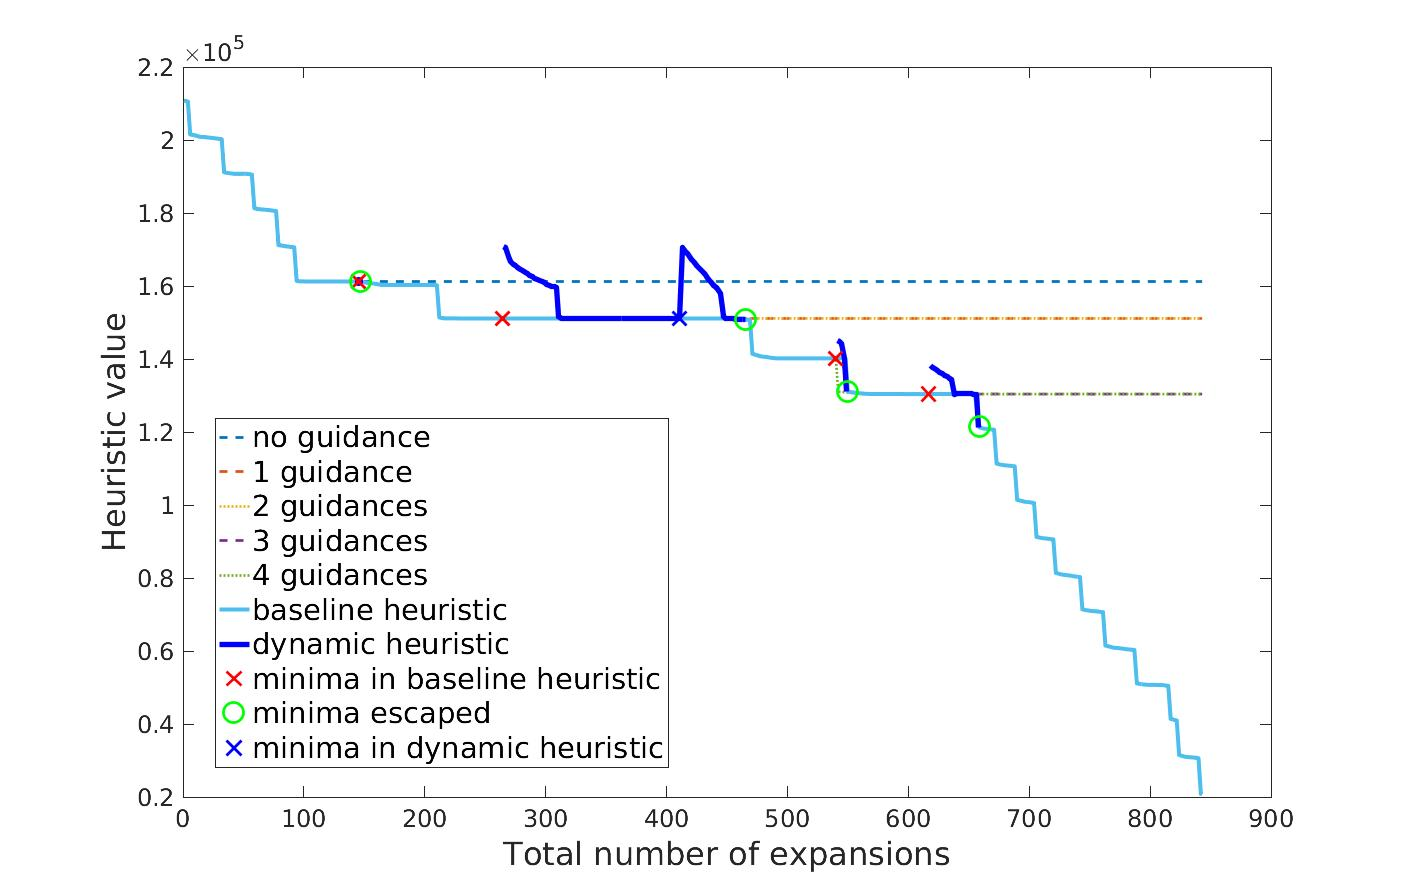
\includegraphics[width=0.4\textwidth]{fig/heuristic_value.jpg}
  	\vspace{-2mm}
  \caption{
		Progress of MHA* with and without user guidance---heuristic values as a function of the number of queue expansions.
		When a local minima is detected (red cross) in the baseline heuristic (cyan), a dynamic heuristic is generated (blue) until the local minima is escaped (green circle) or until a local minima is detected (blue cross) in the dynamic heuristic.
		Plots depicting the baseline heuristic values when only a limited amount of guidance is given demonstrate that without guidance, the planner remains stuck in local minima (we note that as MHA* is complete, it will eventually escape all local minima).
		}
\vspace{-5mm}
   	\label{fig:res}
\end{figure}

While providing promising initial results, our framework is far from being complete.
We are interested in experimenting with alternative forms of user guidance such as providing a \emph{constrained submanifold} of the configuration space. This may be used to guide the humanoid to use the railing while planning the stairs.
%Furthermore, we would like to have a \emph{recursive} implementation of our framework.
%Namely, the planner can be in a local minima while trying to escape a local minima. This should be identified and then the user should either (i)~provide new guidance 
%\os{This is already implemented}
%or 
%(ii)~provide  guidance  toward the previoulsy provided guidance.
Finally, once a guide is given, we want our planner to be able to \emph{generalize} the guidance obtained to future local minima that are similar in nature to the ones encountered.

%\newpage

%\bibliographystyle{plainnat}
\bibliographystyle{abbrv}
\bibliography{bibliography}

\end{document}

%%% Local Variables:
%%% mode: latex
%%% TeX-master: t
%%% End:
